\documentclass[./skripsi.tex]{subfiles}
\begin{document}
\chapter{Hasil Penelitian}
\section{Deskripsi Hasil Penelitian}
\par Hasil penelitian terdiri dari data hasil training CNN, LSTM, dan data hasil testing pada snortIDS. Data Hasil dari LSTM dan CNN merupakan data hasil Training, Testing, dan hasil prediksi dari model \textit{Neural Network}.
\par Data hasil pada sisi CNN melakukan filtrasi packet dengan mendeteksi packet yang berada dalam raw header. Sedangkan data hasil pada sisi LSTM melakukan profiling packet dengan memisahkan deret packet berdasarkan alamat IP yang kemudian dilakukan training.
\par Setiap input data langkah awal yang dilakukan adalah melakukan data mining untuk melihat sumber packet yang dikirim, dan tujuannya. Dan memprediksi apakah data itu masuk atau keluar.
\par Data yang dijadikan input pada sisi CNN adalah seluruh data yang masuk pada host. Sedangkan data yang dijadikan input pada sisi LSTM adalah seluruh data header baik keluar maupun masuk dari host.
\par Proses yang dilakukan untuk memperoleh data hasil adalah dengan menggunakan SnortIDS mengirimkan 10 parameter header dengan payloadnya.
\par Pada sisi service flask akan didefinisikan buffer pada setiap data yang masuk berdasarkan sumber alamat IP nya. Buffer untuk IP ini terbagi menjadi 3 yakni, buffer transmit, receive, dan transceive. Buffer transmit, dan receive yang berkaitan akan digabungkan untuk mendeteksi intrusi pada sisi packet header dengan LSTM. Dan buffer transmit dengan per IP akan digunakan untuk mendeteksi intrusi pada sisi packet payload dengan CNN. 
\section{Hasil Training Data Neural Network}
\par Hasil training data untuk model Neural Network dengan model :
\subsection{Model CNN}
\begin{figure}[H]
    \centering
    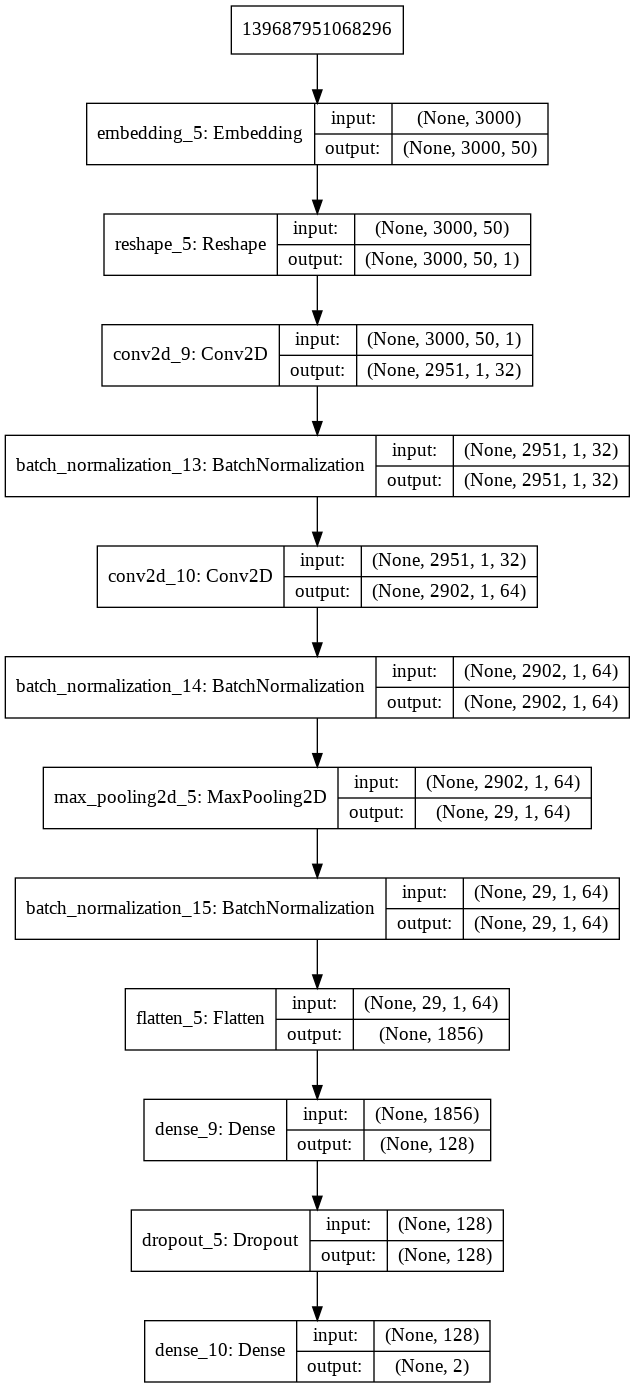
\includegraphics[width=0.5\textwidth]{public/assets/img/CNNModel.png}
    \caption{Model CNN}
    \label{fig:model_cnn}
\end{figure}
\setlength{\textfloatsep}{0.7\baselineskip plus 0.2\baselineskip minus 0.5\baselineskip}
\par Berdasarkan gambar \ref{fig:model_cnn} diatas, pada model CNN terdapat layer Embedding digunakan untuk mengekstraksi fitur dari data input dengan ukuran 2xMTU atau 3000 Byte. Layer selanjutnya adalah layer Reshape yang mengubah ukuran input dari 3000x50 menjadi 3000x50x1 dengan kata lain menginklusi matriks dari matriks 2 dimensi menjadi matriks 3 dimensi dengan ketebalan 1.
\par Layer selanjutnya merupakan layer konvolusi, pada konvolusi pertama dan kedua outputnya di normalisasi dengan BatchNormalization, dan pada Layers konvolusi terakhir dilakukan MaxPooling untuk meniadakan interpretasi yang akan mengurangi rate pendeteksian. Setelah semua konvolusi selesai matriks dinormalisasi lagi sebelum masuk ke layer selanjutnya.
\par Layer selanjutnya merupakan layer untuk deteksi. Pada layer Flatten semua matriks pada layer konvolusi terakhir diubah menjadi vektor. Kemudian setelah itu masuk ke layer Dense atau untuk aktivasi pertama lalu masuk ke Dropout untuk mengurangi neuron irrelevan dari Dense sebelumnya. Kemudian keluaran dari Dropout Layer menjadi input bagi Layer Dense terakhir yang berukuran vektor 2 bit, atau memiliki 2 kelas. Dari kedua kelas ini hanya kategori [0 1] yang dilakukan training data.

\subsection{Model LSTM}
\begin{figure}[H]
    \centering
    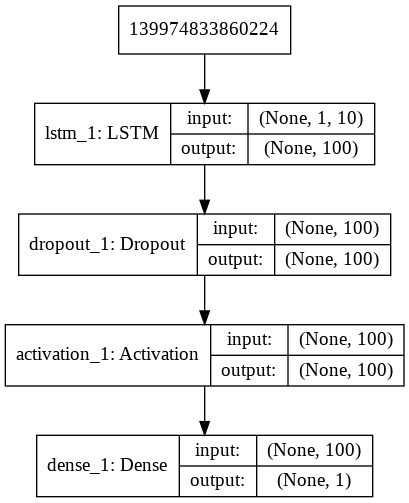
\includegraphics[width=0.5\textwidth]{public/assets/img/LSTMModel.png}
    \caption{Model LSTM}
    \label{fig:lstm_model}
\end{figure}
\par Pada Gambar \ref{fig:lstm_model} model LSTM hanya terdapat layer LSTM sebagai pembaca vektor header dari packet. Dropout untuk menghilangkan neuron yang irrelevan. Layer Activation dimana hasil keluaran Layer sebelumnya diaktivasi dengan menggunakan fungsi aktivasi \textit{softmax} dan Dense dengan ukuran klaster 1, yakni memiliki skalar untuk pendeteksiannya.
\par Untuk proses pendeteksian dengan sentiment analysis neuron Dense berjumlah 1, sedangkan untuk prediksi multivariable neuron Dense berjumlah 10, dimana neuron ini merupakan jumlah parameter pada header packet.
\subsection{Hasil Training Data LSTM}
\par Sistem training data LSTM menggunakan 2 metode yang berbeda yakni \textit{Sentiment Analysis} dan \textit{Multivariate Prediction}. Hasil \textit{training} kedua metode ini memiliki perbedaan dimana pada \textit{Sentiment Analysis} dapat memprediksi apabila variasi dan distribusi variasi pada targetnya merata. Sedangkan pada \textit{Multivariate Prediction} hasil training memiliki karakteristik konvergen yang tinggi karena memperhitungkan dan memprediksi data secara keseluruhan.

\subsubsection{Hasil training Svchosta Botnet dengan Sentiment Analysis LSTM}
\par Untuk Hasil training svchosta dengan sentiment analysis memiliki data sebagai berikut :
\begin{figure}[H]
    \centering
    \buatsubgrafik {public/assets/img/lstms_svchosta_loss.png}{Loss model LSTM svchosta}{.4}
    \buatsubgrafik {public/assets/img/lstms_svchosta_acc.png}{Akurasi model LSTM svchosta}{.4}
    \caption{Loss dan Akurasi model LSTM svchosta Sentiment Analysis}
    \label{fig:lstms_svchosta}
\end{figure}

\par Dari grafik \ref{fig:lstms_svchosta} dapat dilihat sesuai dengan nilai sebelumnya. Kisaran akurasi Loss dari model svchosta test ada di antara 0.016 dan 0.015, sedangkan kisaran akurasi Loss dari model svchosta train ada di antara 0.011 dan 0.012. Hasil akurasi diperoleh dapat diamati juga kisaran train berada di sekitar 0.989, dan kisaran test berada di sekitar 0.985.

\begin{figure}[H]
    \centering
    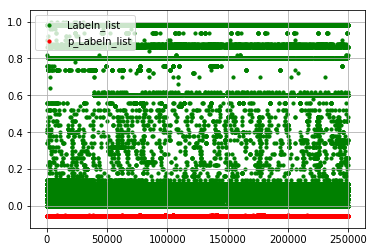
\includegraphics[width=0.5\textwidth]{public/assets/img/lstms_svchosta_pred.png}
    \caption{Prediksi model LSTM svchosta Sentiment Analysis}
    \label{fig:lstms_svchosta_pred}
\end{figure}

\par Dari grafik \ref{fig:lstms_svchosta_pred} diatas dapat dilihat bentuk prediksi \textit{LSTM Sentiment Analysis}. Tampak variasi trafik label yang diperoleh di prediksi hanya bernilai 0, sedangkan beberapa label lain tidak terdeteksi sama sekali. Hal ini dikarenakan jarangnya trafik malware yang ada pada jaringan. Pemberian angka dilakukan pada setiap label yang berbeda. Nilai 0 diperoleh dikarenakan label yang dianalisis bukan merupakan label dari botnet.

% Tabel Hasil Sentiment
\begin{table}[H]
\centering
\caption{Tabel Hasil LSTMS Svchosta}
\begin{tabelkeras}
\hline
0  &  0.015402 &  0.98474 &                 0.015402 &                       1.0 &  0.011336 &  0.98888 &             0.011336 &                   1.0 \\
5  &  0.015288 &  0.98474 &                 0.015288 &                       1.0 &  0.011274 &  0.98888 &             0.011274 &                   1.0 \\
10 &  0.015347 &  0.98474 &                 0.015347 &                       1.0 &  0.011353 &  0.98888 &             0.011353 &                   1.0 \\
15 &  0.015331 &  0.98474 &                 0.015331 &                       1.0 &  0.011340 &  0.98888 &             0.011340 &                   1.0 \\
20 &  0.015695 &  0.98474 &                 0.015695 &                       1.0 &  0.011318 &  0.98888 &             0.011318 &                   1.0 \\
25 &  0.015413 &  0.98474 &                 0.015413 &                       1.0 &  0.011345 &  0.98888 &             0.011345 &                   1.0 \\
30 &  0.015288 &  0.98474 &                 0.015288 &                       1.0 &  0.011383 &  0.98888 &             0.011383 &                   1.0 \\
35 &  0.015349 &  0.98474 &                 0.015349 &                       1.0 &  0.011274 &  0.98888 &             0.011274 &                   1.0 \\
40 &  0.015405 &  0.98474 &                 0.015405 &                       1.0 &  0.011274 &  0.98888 &             0.011274 &                   1.0 \\
45 &  0.015570 &  0.98474 &                 0.015570 &                       1.0 &  0.011395 &  0.98888 &             0.011395 &                   1.0 \\
\hline
\end{tabelkeras}
\label{table:lstms_svchosta}
\end{table}

\par Berdasarkan tabel \ref{table:lstms_svchosta} diatas dapat dilihat tidak terjadi konvergensi pada (Value Loss) VL, (Loss) L, maupun parameter (A) Akurasi. Nilai yang diperoleh di sisi Loss bernilai 0.011 dan akurasi 0.989. Tidak terjadi perubahan setiap epoch. Beberapa parameter terjadi sedikit fluktuasi pada sisi prediksi.

\subsubsection{Hasil Training Neris Botnet dengan Sentiment Analysis LSTM}
\par Untuk Hasil training Neris dengan sentiment analysis memiliki data sebagai berikut :

\begin{figure}[H]
    \centering
    \buatsubgrafik {public/assets/img/lstms_neris_loss.png}{Loss model LSTM neris}{.4}
    \buatsubgrafik {public/assets/img/lstms_neris_acc.png}{Akurasi model LSTM neris}{.4}
    \caption{Loss dan Akurasi model LSTM neris Sentiment Analysis}
    \label{fig:lstms_neris}
\end{figure}

\par Dari grafik \ref{fig:lstms_neris} diatas dapat dilihat sesuai dengan nilai sebelumnya. Hal ini disebabkan karena data yang bernilai malicious pada \textit{header} sangat kecil sehingga dapat diabaikan.

\begin{figure}[H]
    \centering
    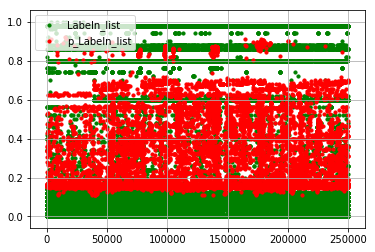
\includegraphics[width=0.5\textwidth]{public/assets/img/lstms_neris_pred.png}
    \caption{Prediksi model LSTM neris Sentiment Analysis}
    \label{fig:lstms_neris_pred}
\end{figure}

\par Dari grafik \ref{fig:lstms_neris_pred}  dapat dilihat bentuk prediksi \textit{LSTM Sentiment Analysis}. Pada sisi loss model dari hasil testing berada di kisaran 0.0108 sampai 0.0112, sedangkan loss di hasil training berada di kisaran 0.0118, dan 0.0116. Pada sisi akurasi model dari hasil testing berada di kisaran 0.9893, sedangkan dari hasil training berada di kisaran 0.9885. Tidak terjadi perubahan pada kedua grafik ini dikarenakan tidak terjadiny a pembelajaran pada model ini.

% Tabel Hasil Sentiment
\begin{table}[H]
\centering
\caption{Tabel Hasil LSTMS Neris}
\begin{tabelkeras}
\hline
0  &  0.010916 &  0.989313 &                 0.010916 &                       1.0 &  0.011702 &  0.988516 &             0.011702 &                   1.0 \\
5  &  0.010751 &  0.989313 &                 0.010751 &                       1.0 &  0.011737 &  0.988516 &             0.011737 &                   1.0 \\
10 &  0.010809 &  0.989313 &                 0.010809 &                       1.0 &  0.011778 &  0.988516 &             0.011778 &                   1.0 \\
15 &  0.010946 &  0.989313 &                 0.010946 &                       1.0 &  0.011678 &  0.988516 &             0.011678 &                   1.0 \\
20 &  0.011027 &  0.989313 &                 0.011027 &                       1.0 &  0.011685 &  0.988516 &             0.011685 &                   1.0 \\
25 &  0.010838 &  0.989313 &                 0.010838 &                       1.0 &  0.011664 &  0.988516 &             0.011664 &                   1.0 \\
30 &  0.010762 &  0.989313 &                 0.010762 &                       1.0 &  0.011652 &  0.988516 &             0.011652 &                   1.0 \\
35 &  0.011100 &  0.989313 &                 0.011100 &                       1.0 &  0.011623 &  0.988516 &             0.011623 &                   1.0 \\
40 &  0.011066 &  0.989313 &                 0.011066 &                       1.0 &  0.011616 &  0.988516 &             0.011616 &                   1.0 \\
45 &  0.010992 &  0.989313 &                 0.010992 &                       1.0 &  0.011733 &  0.988516 &             0.011733 &                   1.0 \\
\hline
\end{tabelkeras}
\label{table:lstms_neris}
\end{table}

\par Berdasarkan tabel \ref{table:lstms_neris} diatas dapat dilihat tidak terjadi konvergensi pada (Value Loss) VL, (Loss) L, maupun parameter (A) Akurasi. Hal ini disebabkan karena tidak terjadi pembelajaran data dikarenakan dataset memiliki label yang tidak seimbang.

\subsubsection{Hasil Training Rbot Botnet dengan Sentiment Analysis LSTM}
\par Untuk Hasil training Rbot dengan sentiment analysis memiliki data sebagai berikut :

\begin{figure}[H]
    \centering
    \buatsubgrafik{public/assets/img/lstms_rbot_loss.png}{Loss model LSTM rbot}{.4}
    \buatsubgrafik{public/assets/img/lstms_rbot_acc.png}{Akurasi model LSTM rbot}{.4}
    \caption{Loss dan Akurasi model LSTM rbot Sentiment Analysis}
    \label{fig:lstms_rbot}
\end{figure}

\par Dari grafik \ref{fig:lstms_rbot} diatas dapat dilihat sesuai dengan nilai sebelumnya. Hal ini disebabkan karena data yang bernilai malicious pada \textit{header} sangat kecil sehingga dapat diabaikan.

\begin{figure}[H]
    \centering
    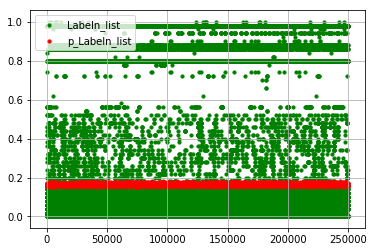
\includegraphics[width=0.5\textwidth]{public/assets/img/lstms_rbot_pred.png}
    \caption{Prediksi model LSTM rbot Sentiment Analysis}
    \label{fig:lstms_rbot_pred}
\end{figure}

\par Dari grafik \ref{fig:lstms_rbot_pred} diatas dapat dilihat bentuk prediksi \textit{LSTM Sentiment Analysis}. Karena saat training tidak terjadi konvergensi, sehingga data prediksi yang diperoleh tidak menunjukkan kecocokan antara hasil prediksi dengan data real.

% Tabel Hasil Sentiment

\begin{table}[H]
\centering
\caption{Tabel Hasil LSTMS RBot}
\begin{tabelkeras}
\hline
0  &  0.025622 &  0.974672 &                 0.025622 &                       1.0 &  0.015825 &  0.984372 &             0.015825 &                   1.0 \\
5  &  0.025387 &  0.974672 &                 0.025387 &                       1.0 &  0.015732 &  0.984372 &             0.015732 &                   1.0 \\
10 &  0.025461 &  0.974672 &                 0.025461 &                       1.0 &  0.015732 &  0.984372 &             0.015732 &                   1.0 \\
15 &  0.025463 &  0.974672 &                 0.025463 &                       1.0 &  0.015892 &  0.984372 &             0.015892 &                   1.0 \\
20 &  0.025491 &  0.974672 &                 0.025491 &                       1.0 &  0.015925 &  0.984372 &             0.015925 &                   1.0 \\
25 &  0.025443 &  0.974672 &                 0.025443 &                       1.0 &  0.015815 &  0.984372 &             0.015815 &                   1.0 \\
30 &  0.025374 &  0.974672 &                 0.025374 &                       1.0 &  0.015709 &  0.984372 &             0.015709 &                   1.0 \\
35 &  0.025417 &  0.974672 &                 0.025417 &                       1.0 &  0.015730 &  0.984372 &             0.015730 &                   1.0 \\
40 &  0.025413 &  0.974672 &                 0.025413 &                       1.0 &  0.015744 &  0.984372 &             0.015744 &                   1.0 \\
45 &  0.025428 &  0.974672 &                 0.025428 &                       1.0 &  0.015821 &  0.984372 &             0.015821 &                   1.0 \\
\hline
\end{tabelkeras}
\label{table:lstms_rbot}
\end{table}

\par Berdasarkan tabel \ref{table:lstms_rbot} diatas dapat dilihat tidak terjadi konvergensi pada (Value Loss) VL, (Loss) L, maupun parameter (A) Akurasi. Hal ini disebabkan karena tidak terjadi pembelajaran data dikarenakan dataset memiliki label yang tidak seimbang.

% Mulai Multivariate Prediction
\subsubsection{Hasil Training svchosta Botnet dengan Multivariate Prediction LSTM}
\par Untuk Hasil training svchosta dengan multivariate prediction memiliki data sebagai berikut :

\begin{figure}[H]
    \buatsubgrafik{public/assets/img/lstmm_svchosta_loss.png}{Loss model LSTM svchosta}{.4}
    \buatsubgrafik{public/assets/img/lstmm_svchosta_acc.png}{Akurasi model LSTM svchosta}{.4}
    \caption{Loss dan Akurasi model LSTM svchosta}
    \label{fig:lstmm_svchosta}
\end{figure}

\par Berdasarkan dari grafik \ref{fig:lstmm_svchosta} diatas dapat diamati bahwa hasil training konvergen. Hal ini dapat dilihat dari grafik yang mengalami pemusatan pada satu sumbu y baik pada grafik \textit{Loss} maupun pada grafik \textit{Accuracy}.

% Grafik sepuluh prediksi
\begin{figure}[H]
    \centering
    \buatsubgrafik {public/assets/img/lstmm_svchosta_pred1.png}{Prediksi Svchosta 1}{.4}
    \buatsubgrafik {public/assets/img/lstmm_svchosta_pred2.png}{Prediksi Svchosta 2}{.4}
    \buatsubgrafik {public/assets/img/lstmm_svchosta_pred3.png}{Prediksi Svchosta 3}{.4}
    \buatsubgrafik {public/assets/img/lstmm_svchosta_pred4.png}{Prediksi Svchosta 4}{.4}
    \buatsubgrafik {public/assets/img/lstmm_svchosta_pred5.png}{Prediksi Svchosta 5}{.4}
    \buatsubgrafik {public/assets/img/lstmm_svchosta_pred6.png}{Prediksi Svchosta 6}{.4}
    \buatsubgrafik {public/assets/img/lstmm_svchosta_pred7.png}{Prediksi Svchosta 7}{.4}
    \buatsubgrafik {public/assets/img/lstmm_svchosta_pred8.png}{Prediksi Svchosta 8}{.4}
    \buatsubgrafik {public/assets/img/lstmm_svchosta_pred9.png}{Prediksi Svchosta 9}{.4}
    \buatsubgrafik {public/assets/img/lstmm_svchosta_pred10.png}{Prediksi Svchosta 10}{.4}
    \caption{Grafik Prediksi Svchosta}
    \label{fig:lstmm_svchosta_pred}
\end{figure}

\par Berdasarakan grafik \ref{fig:lstmm_svchosta_pred} keseluruhan dari hasil prediksi kesepuluh parameter \textit{LSTM Multivariate Prediction}, dapat dilihat bahwa pada beberapa parameter prediksi terdapat beberapa parmaeter yang berhasil di prediksi dan beberapa parameter pula yang tidak dapat terdeteksi.

% Tabel Hasil
\begin{table}[H]
\centering
\caption{Tabel Hasil LSTMM Svc}
\begin{tabelkeras}
\hline
0  &  0.076987 &  0.764155 &                 0.076987 &                  0.764155 &  0.128025 &  0.506444 &             0.128025 &              0.506444 \\
5  &  0.034513 &  0.373282 &                 0.034513 &                  0.373282 &  0.048499 &  0.708092 &             0.048499 &              0.708092 \\
10 &  0.033781 &  0.380621 &                 0.033781 &                  0.380621 &  0.045702 &  0.702732 &             0.045702 &              0.702732 \\
15 &  0.032518 &  0.378274 &                 0.032518 &                  0.378274 &  0.044133 &  0.698664 &             0.044133 &              0.698664 \\
20 &  0.031653 &  0.376445 &                 0.031653 &                  0.376445 &  0.042929 &  0.696064 &             0.042929 &              0.696064 \\
25 &  0.031494 &  0.376694 &                 0.031494 &                  0.376694 &  0.042119 &  0.696388 &             0.042119 &              0.696388 \\
30 &  0.029571 &  0.376736 &                 0.029571 &                  0.376736 &  0.041559 &  0.694804 &             0.041559 &              0.694804 \\
35 &  0.029802 &  0.375568 &                 0.029802 &                  0.375568 &  0.041111 &  0.696844 &             0.041111 &              0.696844 \\
40 &  0.029912 &  0.377669 &                 0.029912 &                  0.377669 &  0.040611 &  0.695416 &             0.040611 &              0.695416 \\
45 &  0.028958 &  0.376280 &                 0.028958 &                  0.376280 &  0.040329 &  0.694196 &             0.040329 &              0.694196 \\
\hline
\end{tabelkeras}
\label{table:lstmm_svchosta}
\end{table}

\par Berdasarkan tabel \ref{table:lstmm_svchosta} diatas dapat diamati bahwa penurunan Loss terjadi dan peningkatan terjadi. Pada sisi akurasi dapat dilihat bahwa akurasi tertinggi yang dicapai model adalah 0.7. Hal ini dikarenakan beberapa parameter tidak mempengaruhi satu sama lain, namun berdasarkan keseluruhan hasil prediksi yang diperoleh dapat digunakan untuk melakukan profiling.

\subsubsection{Hasil Training Neris Botnet dengan Multivariate Prediction LSTM}

\begin{figure}[H]
    \centering
    \buatsubgrafik {public/assets/img/lstmm_neris_loss.png}{Loss model LSTM neris}{.4}
    \buatsubgrafik {public/assets/img/lstmm_neris_acc.png}{Akurasi model LSTM neris}{.4}
    \caption{Loss dan Akurasi model LSTM neris}
    \label{fig:lstmm_neris}
\end{figure}

\par Berdasarkan dari grafik \ref{fig:lstmm_neris} diatas dapat diamati bahwa hasil training konvergen. Hal ini dapat dilihat dari grafik yang mengalami pemusatan pada satu sumbu y baik pada grafik \textit{Loss} maupun pada grafik \textit{Accuracy}.

% Grafik sepuluh prediksi
\begin{figure}[H]
    \centering
    \buatsubgrafik {public/assets/img/lstmm_neris_pred1.png}{Prediksi Neris 1}{.4}
    \buatsubgrafik {public/assets/img/lstmm_neris_pred2.png}{Prediksi Neris 2}{.4}
    \buatsubgrafik {public/assets/img/lstmm_neris_pred3.png}{Prediksi Neris 3}{.4}
    \buatsubgrafik {public/assets/img/lstmm_neris_pred4.png}{Prediksi Neris 4}{.4}
    \buatsubgrafik {public/assets/img/lstmm_neris_pred5.png}{Prediksi Neris 5}{.4}
    \buatsubgrafik {public/assets/img/lstmm_neris_pred6.png}{Prediksi Neris 6}{.4}
    \buatsubgrafik {public/assets/img/lstmm_neris_pred7.png}{Prediksi Neris 7}{.4}
    \buatsubgrafik {public/assets/img/lstmm_neris_pred8.png}{Prediksi Neris 8}{.4}
    \buatsubgrafik {public/assets/img/lstmm_neris_pred9.png}{Prediksi Neris 9}{.4}
    \buatsubgrafik {public/assets/img/lstmm_neris_pred10.png}{Prediksi Neris 10}{.4}
    \caption{Grafik Prediksi Neris}
    \label{fig:lstmm_neris_pred}
\end{figure}

\par Berdasarakan grafik \ref{fig:lstmm_neris_pred} keseluruhan dari hasil prediksi kesepuluh parameter \textit{LSTM Multivariate Prediction}, dapat dilihat bahwa pada beberapa parameter prediksi terdapat beberapa parmaeter yang berhasil di prediksi dan beberapa parameter pula yang tidak dapat terdeteksi.

% Tabel Hasil
\begin{table}[H]
\centering
\caption{Tabel Hasil LSTMM Neris}
\begin{tabelkeras}
\hline
0  &  0.065239 &  0.654737 &                 0.065239 &                  0.654737 &  0.119845 &  0.449928 &             0.119845 &              0.449928 \\
5  &  0.034839 &  0.733986 &                 0.034839 &                  0.733986 &  0.046002 &  0.741092 &             0.046002 &              0.741092 \\
10 &  0.031048 &  0.442449 &                 0.031048 &                  0.442449 &  0.040226 &  0.743360 &             0.040226 &              0.743360 \\
15 &  0.029231 &  0.388196 &                 0.029231 &                  0.388196 &  0.037856 &  0.741544 &             0.037856 &              0.741544 \\
20 &  0.028663 &  0.376175 &                 0.028663 &                  0.376175 &  0.036085 &  0.739152 &             0.036085 &              0.739152 \\
25 &  0.028420 &  0.373686 &                 0.028420 &                  0.373686 &  0.034885 &  0.740980 &             0.034885 &              0.740980 \\
30 &  0.027671 &  0.381238 &                 0.027671 &                  0.381238 &  0.034157 &  0.741424 &             0.034157 &              0.741424 \\
35 &  0.028124 &  0.385267 &                 0.028124 &                  0.385267 &  0.033609 &  0.739756 &             0.033609 &              0.739756 \\
40 &  0.028225 &  0.383293 &                 0.028225 &                  0.383293 &  0.033262 &  0.738816 &             0.033262 &              0.738816 \\
45 &  0.028852 &  0.377458 &                 0.028852 &                  0.377458 &  0.032910 &  0.739264 &             0.032910 &              0.739264 \\
\hline
\end{tabelkeras}
\label{table:lstmm_neris}
\end{table}

\par Berdasarkan tabel \ref{table:lstmm_neris} diatas dapat diamati bahwa penurunan Loss terjadi dan peningkatan terjadi. Pada sisi akurasi dapat dilihat bahwa akurasi tertinggi yang dicapai model adalah 0.75. Hal ini dikarenakan beberapa parameter tidak mempengaruhi satu sama lain, namun berdasarkan keseluruhan hasil prediksi yang diperoleh dapat digunakan untuk melakukan profiling.

\subsubsection{Hasil Training Rbot Botnet dengan Multivariate Prediction LSTM}

\begin{figure}[H]
    \centering
    \buatsubgrafik {public/assets/img/lstmm_rbot_loss.png}{Loss model LSTM rbot}{.2}
    \buatsubgrafik {public/assets/img/lstmm_rbot_acc.png}{Akurasi model LSTM rbot}{.2}
    \caption{Loss dan Akurasi model LSTM rbot}
    \label{fig:lstmm_rbot}
\end{figure}

\par Berdasarkan dari grafik \ref{fig:lstmm_rbot} diatas dapat diamati bahwa hasil training konvergen. Hal ini dapat dilihat dari grafik yang mengalami pemusatan pada satu sumbu y baik pada grafik \textit{Loss} maupun pada grafik \textit{Accuracy}.

% Grafik sepuluh prediksi
\begin{figure}
    \centering
    \buatsubgrafik {public/assets/img/lstmm_rbot_pred1.png}{Prediksi Rbot 1}{.4}
    \buatsubgrafik {public/assets/img/lstmm_rbot_pred2.png}{Prediksi Rbot 2}{.4}
    \buatsubgrafik {public/assets/img/lstmm_rbot_pred3.png}{Prediksi Rbot 3}{.4}
    \buatsubgrafik {public/assets/img/lstmm_rbot_pred4.png}{Prediksi Rbot 4}{.4}
    \buatsubgrafik {public/assets/img/lstmm_rbot_pred5.png}{Prediksi Rbot 5}{.4}
    \buatsubgrafik {public/assets/img/lstmm_rbot_pred6.png}{Prediksi Rbot 6}{.4}
    \buatsubgrafik {public/assets/img/lstmm_rbot_pred7.png}{Prediksi Rbot 7}{.4}
    \buatsubgrafik {public/assets/img/lstmm_rbot_pred8.png}{Prediksi Rbot 8}{.4}
    \buatsubgrafik {public/assets/img/lstmm_rbot_pred9.png}{Prediksi Rbot 9}{.4}
    \buatsubgrafik {public/assets/img/lstmm_rbot_pred10.png}{Prediksi Rbot 10}{.4}
    \caption{Grafik Prediksi RBot}
    \label{fig:lstmm_rbot_pred}
\end{figure}

\par Berdasarakan grafik \ref{fig:lstmm_rbot_pred} keseluruhan dari hasil prediksi kesepuluh parameter \textit{LSTM Multivariate Prediction}, dapat dilihat bahwa pada beberapa parameter prediksi terdapat beberapa parmaeter yang berhasil di prediksi dan beberapa parameter pula yang tidak dapat terdeteksi.

% Tabel Hasil
\begin{table}[H]
\centering
\caption{Tabel Hasil LSTMM Rbot}
\begin{tabelkeras}
\hline
0  &  0.096960 &  0.717496 &                 0.096960 &                  0.717496 &  0.124205 &  0.469576 &             0.124205 &              0.469576 \\
5  &  0.039409 &  0.815303 &                 0.039409 &                  0.815303 &  0.046257 &  0.731320 &             0.046257 &              0.731320 \\
10 &  0.037089 &  0.813762 &                 0.037089 &                  0.813762 &  0.043225 &  0.733896 &             0.043225 &              0.733896 \\
15 &  0.036373 &  0.778298 &                 0.036373 &                  0.778298 &  0.041665 &  0.736736 &             0.041665 &              0.736736 \\
20 &  0.036282 &  0.803957 &                 0.036282 &                  0.803957 &  0.040376 &  0.743860 &             0.040376 &              0.743860 \\
25 &  0.035489 &  0.702191 &                 0.035489 &                  0.702191 &  0.039543 &  0.745740 &             0.039543 &              0.745740 \\
30 &  0.034391 &  0.765884 &                 0.034391 &                  0.765884 &  0.038935 &  0.744652 &             0.038935 &              0.744652 \\
35 &  0.034246 &  0.698371 &                 0.034246 &                  0.698371 &  0.038311 &  0.747672 &             0.038311 &              0.747672 \\
40 &  0.033922 &  0.736452 &                 0.033922 &                  0.736452 &  0.038004 &  0.747848 &             0.038004 &              0.747848 \\
45 &  0.033341 &  0.700033 &                 0.033341 &                  0.700033 &  0.037738 &  0.747188 &             0.037738 &              0.747188 \\
\hline
\end{tabelkeras}
\label{table:lstmm_rbot}
\end{table}

\par Berdasarkan tabel \ref{table:lstmm_rbot} diatas dapat diamati bahwa penurunan Loss terjadi dan peningkatan terjadi. Pada sisi akurasi dapat dilihat bahwa akurasi tertinggi yang dicapai model adalah 0.75. Hal ini dikarenakan beberapa parameter tidak mempengaruhi satu sama lain, namun berdasarkan keseluruhan hasil prediksi yang diperoleh dapat digunakan untuk melakukan profiling.

\subsubsection{Hasil Training LSTM Svchosta 4 Directional Header}
% Grafik model

\begin{figure}[H]
    \centering
    \buatsubgrafik{public/assets/img/lstm4_svchosta_loss.png}{Loss model LSTM4 svchosta}{.4}
    \buatsubgrafik{public/assets/img/lstm4_svchosta_acc.png}{Akurasi model LSTM4 svchosta}{.4}
    \caption{Loss dan Akurasi model LSTM4 Svchosta}
    \label{fig:lstm4_svchosta}
\end{figure}

\par Berdasarkan grafik training \ref{fig:lstm4_svchosta} diatas, dapat dilihat bahwa pada sisi loss terjadi konvergensi baik pada sisi \textit{Loss} maupun pada sisi \textit{Akurasi}. Semakin banyak \textit{epoch} yang terjadi maka semakin kecil \textit{Loss} yang diperoleh. Semakin banyak \textit{epoch} yang terjadi maka semakin tinggi \textit{Accuracy} yang diperoleh.

% Grafik prediksi IP
\begin{figure}[H]
    \centering
    \buatsubgrafik{public/assets/img/lstm4_svchosta_pred1.png}{Prediksi IPSrc model LSTM4 svchosta}{.4}
    \buatsubgrafik{public/assets/img/lstm4_svchosta_pred2.png}{Prediksi IPDst model LSTM4 svchosta}{.4}
    \caption{Prediksi IP Address model LSTM4 svchosta}
    \label{fig:lstm4_svchosta_pred1}
\end{figure}

\par Berdasalkan grafik hasil prediksi \ref{fig:lstm4_svchosta_pred1} mengambil 500 sampel dari dataset dapat diamati bahwa hampir secara keseluruhan hasil prediksi cocok dengan data yang di inputkan. Grafik prediksi \textbf{IPSrc} memiliki divergensi yang tinggi berarti banyak IP yang mengakses Server. Sedangkan Grafik IPDst yang lurus menandakan hanya ada satu alamat IP yang dituju yakni alamat IP Server.

% Grafik prediksi Port

\begin{figure}
    \centering
    \buatsubgrafik{public/assets/img/lstm4_svchosta_pred3.png}{Prediksi PortSrc model svchosta}{.4}
    \buatsubgrafik{public/assets/img/lstm4_svchosta_pred4.png}{Prediksi PortDst model LSTM4 svchosta}{.4}
    \caption{Prediksi Port model LSTM4 svchosta}
    \label{fig:lstm4_svchosta_pred2}
\end{figure}

\par Berdasarkan grafik hasil prediksi \ref{fig:lstm4_svchosta_pred2} mengambil 500 sampel dari dataset dapat diamati bahwa hampir secara keseluruhan hasil prediksi cocok dengan data yang di inputkan. Grafik prediksi \textbf{PortSrc} memiliki divergensi yang tinggi berarti banyak Port sumber yang mengakses server. Sedangkan Grafik PortDst yang lurus menandakan hanya ada satu Port yang dituju yakni Port HTTP.

% Tabel Hasil
\begin{table}[H]
\centering
\caption{Tabel Hasil LSTM4 Svchosta}
\begin{tabelkeras}
\hline
0   &  0.432725 &    0.000 &                 0.432725 &                     0.000 &  0.445629 &  0.000 &             0.445629 &                 0.000 \\
100 &  0.038453 &    0.646 &                 0.038453 &                     0.646 &  0.039711 &  0.650 &             0.039711 &                 0.650 \\
200 &  0.037909 &    0.982 &                 0.037909 &                     0.982 &  0.038660 &  0.814 &             0.038660 &                 0.814 \\
300 &  0.036691 &    0.670 &                 0.036691 &                     0.670 &  0.037372 &  0.772 &             0.037372 &                 0.772 \\
400 &  0.032788 &    0.670 &                 0.032788 &                     0.670 &  0.033537 &  0.778 &             0.033537 &                 0.778 \\
500 &  0.025009 &    0.672 &                 0.025009 &                     0.672 &  0.025460 &  0.810 &             0.025460 &                 0.810 \\
600 &  0.012822 &    0.982 &                 0.012822 &                     0.982 &  0.014406 &  0.856 &             0.014406 &                 0.856 \\
700 &  0.004456 &    0.982 &                 0.004456 &                     0.982 &  0.007659 &  0.846 &             0.007659 &                 0.846 \\
800 &  0.002419 &    0.672 &                 0.002419 &                     0.672 &  0.006625 &  0.868 &             0.006625 &                 0.868 \\
900 &  0.002374 &    0.982 &                 0.002374 &                     0.982 &  0.006360 &  0.848 &             0.006360 &                 0.848 \\
\hline
\end{tabelkeras}
\label{table:lstm4_svchosta}
\end{table}

\par Berdasarkan tabel \ref{table:lstm4_svchosta} diatas dapat diamati bahwa seiring dengan meningkatnya jumlah epoch Nilai \textit{Loss} baik \textit{Value Loss} maupun \textit{Loss} menurun. Begitu pula dengan meningkatnya jumlah epoch Nilai \textit{Accuracy} baik \textit{Value Accuracy} maupun \textit{Accuracy}. Dapat diamati pada tabel diatas akurasi tertinggi yang dicapai adalah 98.2\% pada sisi testing dan 84.8\%.

\subsubsection{Hasil Training LSTM Neris 4 Directional Header}
% Grafik model
\begin{figure}
    \centering
    \buatsubgrafik{public/assets/img/lstm4_neris_loss.png}{Loss model LSTM4 Neris}{.4}
    \buatsubgrafik{public/assets/img/lstm4_neris_acc.png}{Akuasi model LSTM4 Neris}{.4}
    \caption{Loss dan Akurasi model LSTM4 Neris}
    \label{fig:lstm4_neris}
\end{figure}

\par Berdasarkan grafik hasil training \ref{fig:lstm4_neris} diatas dapat dilihat bahwa pada sisi loss terjadi konvergensi baik pada sisi \textit{Loss} maupun pada sisi \textit{Akurasi}. Semakin banyak \textit{epoch} yang terjadi maka semakin kecil \textit{Loss} yang diperoleh. Semakin banyak \textit{epoch} yang terjadi maka semakin tinggi \textit{Accuracy} yang diperoleh.

% Grafik prediksi IP
\begin{figure}
    \centering
    \buatsubgrafik{public/assets/img/lstm4_neris_pred1.png}{Prediksi IPSrc model LSTM4 Neris}{.4}
    \buatsubgrafik{public/assets/img/lstm4_neris_pred2.png}{Prediksi IPDst model LSTM4 Neris}{.4}
    \caption{Prediksi IP Address model LSTM4 Neris}
    \label{fig:lstm4_neris_pred1}
\end{figure}

\par Berdasalkan grafik hasil prediksi \ref{fig:lstm4_neris_pred1} mengambil 500 sampel dari dataset dapat diamati bahwa hampir secara keseluruhan hasil prediksi cocok dengan data yang di inputkan. Grafik prediksi \textbf{IPSrc} memiliki divergensi yang tinggi berarti banyak IP yang mengakses Server. Sedangkan Grafik IPDst yang lurus menandakan hanya ada satu alamat IP yang dituju yakni alamat IP Server.

% Grafik prediksi Port
\begin{figure}
    \centering
    \buatsubgrafik{public/assets/img/lstm4_neris_pred3.png}{Prediksi PortSrc model LSTM4 Neris}{.4}
    \buatsubgrafik{public/assets/img/lstm4_neris_pred3.png}{Prediksi PortSrc model LSTM4 Neris}{.4}
    \caption{Prediksi Port model LSTM4 Neris}
    \label{fig:lstm4_neris_pred2}
\end{figure}


\par Berdasarkan grafik hasil prediksi \ref{fig:lstm4_neris_pred2} mengambil 500 sampel dari dataset dapat diamati bahwa hampir secara keseluruhan hasil prediksi cocok dengan data yang di inputkan. Grafik prediksi \textbf{PortSrc} memiliki divergensi yang tinggi berarti banyak Port sumber yang mengakses server. Sedangkan Grafik PortDst yang lurus menandakan hanya ada satu Port yang dituju yakni Port HTTP.

% Tabel Hasil
\begin{table}[H]
\centering
\caption{Tabel Hasil LSTM4 Neris}
\begin{tabelkeras}
\hline
0   &  0.399342 &    0.000 &                 0.399342 &                      2.464162 &  0.405103 &  0.120 &             0.405103 &                  2.539193 \\
100 &  0.049418 &    0.610 &                 0.049418 &                      2.268167 &  0.050036 &  0.642 &             0.050036 &                  2.260185 \\
200 &  0.048140 &    0.826 &                 0.048140 &                      2.266545 &  0.048374 &  0.882 &             0.048374 &                  2.258518 \\
300 &  0.042422 &    0.786 &                 0.042422 &                      2.258401 &  0.041996 &  0.856 &             0.041996 &                  2.249844 \\
400 &  0.026611 &    0.806 &                 0.026611 &                      2.243014 &  0.024903 &  0.898 &             0.024903 &                  2.234774 \\
500 &  0.018720 &    0.980 &                 0.018720 &                      2.237860 &  0.018771 &  0.936 &             0.018771 &                  2.230748 \\
600 &  0.012459 &    0.984 &                 0.012459 &                      2.232215 &  0.013559 &  0.938 &             0.013559 &                  2.226480 \\
700 &  0.006294 &    0.990 &                 0.006294 &                      2.227622 &  0.008677 &  0.936 &             0.008677 &                  2.223640 \\
800 &  0.004994 &    0.990 &                 0.004994 &                      2.227298 &  0.008039 &  0.934 &             0.008039 &                  2.223908 \\
900 &  0.004327 &    0.830 &                 0.004327 &                      2.227232 &  0.007939 &  0.930 &             0.007939 &                  2.223906 \\
\hline
\end{tabelkeras}
\label{table:lstm4_neris}
\end{table}

\par Berdasarkan tabel \ref{table:lstm4_neris} diatas dapat diamati bahwa seiring dengan meningkatnya jumlah epoch Nilai \textit{Loss} baik \textit{Value Loss} maupun \textit{Loss} menurun. Begitu pula dengan meningkatnya jumlah epoch Nilai \textit{Accuracy} baik \textit{Value Accuracy} maupun \textit{Accuracy}. Dapat diamati pada tabel diatas akurasi tertinggi yang dicapai adalah 94.0\% pada sisi testing dan 83.0\%.

\subsubsection{Hasil Training LSTM Rbot 4 Directional Header}
\begin{figure}[H]
    \centering
    \buatsubgrafik{public/assets/img/lstm4_rbot_loss.png}{Loss model LSTM4 Rbot}{.4}
    \buatsubgrafik{public/assets/img/lstm4_rbot_acc.png}{Akurasi model LSTM4 Rbot}{.4}
    \caption{Loss dan Akurasi model LSTM4 Rbot}
    \label{fig:lstm4_rbot}
\end{figure}

\par Berdasarkan grafik hasil training \ref{fig:lstm4_rbot} diatas dapat dilihat bahwa pada sisi loss terjadi konvergensi baik pada sisi \textit{Loss} maupun pada sisi \textit{Akurasi}. Semakin banyak \textit{epoch} yang terjadi maka semakin kecil \textit{Loss} yang diperoleh. Semakin banyak \textit{epoch} yang terjadi maka semakin tinggi \textit{Accuracy} yang diperoleh.

% Grafik prediksi IP
\begin{figure}[H]
    \centering
    \buatsubgrafik{public/assets/img/lstm4_rbot_pred1.png}{Prediksi IPSrc model LSTM4 rbot}{.4}
    \buatsubgrafik{public/assets/img/lstm4_rbot_pred2.png}{Prediksi IPDst model LSTM4 rbot}{.4}
    \caption{Prediksi IP Address model LSTM 4 rbot}
    \label{fig:lstm4_rbot_pred1}
\end{figure}

\par Berdasalkan grafik hasil prediksi \ref{fig:lstm4_rbot_pred1} mengambil 500 sampel dari dataset dapat diamati bahwa hampir secara keseluruhan hasil prediksi cocok dengan data yang di inputkan. Grafik prediksi \textbf{IPSrc} memiliki divergensi yang tinggi berarti banyak IP yang mengakses Server. Sedangkan Grafik IPDst yang lurus menandakan hanya ada satu alamat IP yang dituju yakni alamat IP Server.

% Grafik prediksi Port
\begin{figure}[H]
    \centering
    \buatsubgrafik{public/assets/img/lstm4_rbot_pred3.png}{Prediksi PortSrc model LSTM4 Rbot}{.4}
    \buatsubgrafik{public/assets/img/lstm4_rbot_pred4.png}{Prediksi PortDst model LSTM4 Rbot}{.4}
    \caption{Prediksi Port model LSTM4 Rbot}
    \label{fig:lstm4_rbot_pred2}
\end{figure}

\par Berdasarkan grafik hasil prediksi \ref{fig:lstm4_rbot_pred2} mengambil 500 sampel dari dataset dapat diamati bahwa hampir secara keseluruhan hasil prediksi cocok dengan data yang di inputkan. Grafik prediksi \textbf{PortSrc} memiliki divergensi yang tinggi berarti banyak Port sumber yang mengakses server. Sedangkan Grafik PortDst yang lurus menandakan hanya ada satu Port yang dituju yakni Port HTTP.


% Tabel Hasil
\begin{table}[H]
\centering
\caption{Tabel Hasil LSTM4 Rbot}
\begin{tabelkeras}
\hline
0   &  0.393062 &    0.812 &                 0.393062 &                      2.264847 &  0.395210 &  0.582 &             0.395210 &                  4.385572 \\
100 &  0.019342 &    0.980 &                 0.019342 &                      2.139255 &  0.041992 &  0.684 &             0.041992 &                  2.115251 \\
200 &  0.019122 &    0.996 &                 0.019122 &                      2.138949 &  0.041096 &  0.838 &             0.041096 &                  2.114622 \\
300 &  0.018246 &    0.994 &                 0.018246 &                      2.137809 &  0.039282 &  0.856 &             0.039282 &                  2.112313 \\
400 &  0.015216 &    0.994 &                 0.015216 &                      2.134190 &  0.032752 &  0.832 &             0.032752 &                  2.105142 \\
500 &  0.007832 &    0.998 &                 0.007832 &                      2.129096 &  0.019392 &  0.816 &             0.019392 &                  2.096398 \\
600 &  0.005506 &    0.330 &                 0.005506 &                      2.128211 &  0.016743 &  0.806 &             0.016743 &                  2.094837 \\
700 &  0.004807 &    0.328 &                 0.004807 &                      2.127276 &  0.014481 &  0.810 &             0.014481 &                  2.092351 \\
800 &  0.003952 &    0.328 &                 0.003952 &                      2.126126 &  0.010795 &  0.812 &             0.010795 &                  2.088924 \\
900 &  0.002218 &    0.330 &                 0.002218 &                      2.125234 &  0.007115 &  0.856 &             0.007115 &                  2.086706 \\
\hline
\end{tabelkeras}
\label{table:lstm4_rbot}
\end{table}

\par Berdasarkan tabel \ref{table:lstm4_rbot} diatas dapat diamati bahwa seiring dengan meningkatnya jumlah epoch Nilai \textit{Loss} baik \textit{Value Loss} maupun \textit{Loss} menurun. Begitu pula dengan meningkatnya jumlah epoch Nilai \textit{Accuracy} baik \textit{Value Accuracy} maupun \textit{Accuracy}. Dapat diamati pada tabel diatas akurasi tertinggi yang dicapai adalah 94.0\% pada sisi testing dan 83.0\%.

\subsection{Hasil Training Data CNN}
\par Pada jaringan CNN terjadi proses filter packet payload. Disini ditentukan apakah payload mengandung virus atau tidak. Proses training dilakukan dengan mengubah-ubah parameter learning\_rate. Hal ini dilakukan untuk mengamati perubahan konvergensi proses training dan testing dari CNN.

% Grafik
\newcolumntype{Y}{>{\centering\arraybackslash}X}
% BEGIN TABEL
\subsubsection{Hasil Training CNN Svchosta}
\begin{table}[H]
\centering
\caption{Tabel Hasil Training CNN Svchosta}
\begin{tabularx}{\textwidth}{|*{9}{Y|}}
\hline
    \multirow{2}{*}{Epoch} 
  & \multicolumn{4}{c|}{Akurasi}
  & \multicolumn{4}{c|}{Loss} \\
\cline{2-9}
   &      1e-1 &      1e-2 &      1e-3 &      1e-4 &      1e-1 &      1e-2 &      1e-3 &      1e-4 \\
\cline{1-9}
0  & 0.800 & 0.798 & 0.794 & 0.206 & 0.515 & 0.537 & 0.604 & 0.893 \\
5  & 1.000 & 0.998 & 0.889 & 0.229 & 0.007 & 0.057 & 0.453 & 0.816 \\
10 & 1.000 & 1.000 & 0.950 & 0.308 & 0.003 & 0.027 & 0.337 & 0.750 \\
15 & 1.000 & 1.000 & 0.973 & 0.438 & 0.002 & 0.018 & 0.255 & 0.691 \\
20 & 1.000 & 1.000 & 0.980 & 0.587 & 0.001 & 0.013 & 0.198 & 0.645 \\
25 & 1.000 & 1.000 & 0.984 & 0.741 & 0.001 & 0.011 & 0.160 & 0.596 \\
30 & 1.000 & 1.000 & 0.991 & 0.873 & 0.001 & 0.009 & 0.131 & 0.556 \\
35 & 1.000 & 1.000 & 0.993 & 0.941 & 0.001 & 0.008 & 0.110 & 0.518 \\
40 & 1.000 & 1.000 & 0.995 & 0.973 & 0.001 & 0.007 & 0.096 & 0.485 \\
45 & 1.000 & 1.000 & 0.995 & 0.986 & 0.001 & 0.006 & 0.083 & 0.455 \\
\hline
\end{tabularx}
\label{table:cnn_svchosta_train}
\end{table}
\par Dapat dilihat dari tabel hasil train \ref{table:cnn_svchosta_train}  diatas, semakin banyak epoch maka semakin tinggi akurasi dan semakin rendah loss nya. Lama akurasi mencapai titik tertinggi, dan loss mencapai titik terendah ditentukan oleh \textit{learning rate} .

\par Dapat dilihat berdasarkan parameter \textit{learning rate}, dimana semakin besar nilai \textit{learning rate} maka semakin cepat pula akurasi mencapai titik tertinggi, dan loss mencapai titik terendah.
\begin{table}[H]
\centering
\caption{Tabel Hasil Testing CNN Svchosta}
\begin{tabularx}{\textwidth}{|*{9}{Y|}}
\hline
    \multirow{2}{*}{Epoch} 
  & \multicolumn{4}{c|}{Akurasi}
  & \multicolumn{4}{c|}{Loss} \\
\cline{2-9}
   &      1e-1 &      1e-2 &      1e-3 &      1e-4 &      1e-1 &      1e-2 &      1e-3 &      1e-4 \\
\cline{1-9}
0  & 0.980 & 0.953 & 0.861 & 0.141 & 0.234 & 0.267 & 0.551 & 0.917 \\
5  & 1.000 & 1.000 & 0.920 & 0.169 & 0.008 & 0.050 & 0.417 & 0.832 \\
10 & 1.000 & 1.000 & 0.966 & 0.277 & 0.003 & 0.024 & 0.306 & 0.762 \\
15 & 1.000 & 1.000 & 0.981 & 0.407 & 0.002 & 0.016 & 0.228 & 0.701 \\
20 & 1.000 & 1.000 & 0.987 & 0.601 & 0.001 & 0.013 & 0.176 & 0.649 \\
25 & 1.000 & 1.000 & 0.991 & 0.782 & 0.001 & 0.009 & 0.140 & 0.603 \\
30 & 1.000 & 1.000 & 0.995 & 0.900 & 0.001 & 0.008 & 0.115 & 0.561 \\
35 & 1.000 & 1.000 & 0.997 & 0.959 & 0.001 & 0.007 & 0.096 & 0.523 \\
40 & 1.000 & 1.000 & 0.997 & 0.981 & 0.001 & 0.006 & 0.083 & 0.488 \\
45 & 1.000 & 1.000 & 0.997 & 0.991 & 0.001 & 0.005 & 0.072 & 0.456 \\
\hline
\end{tabularx}
\label{table:cnn_svchosta_test}
\end{table}
\par Dapat dilihat dari tabel hasil test \ref{table:cnn_svchosta_test} diatas, semakin banyak epoch maka semakin tinggi akurasi dan semakin rendah loss nya. Lama akurasi mencapai titik tertinggi, dan loss mencapai titik terendah ditentukan oleh \textit{learning rate}.
\par Dapat dilihat berdasarkan parameter \textit{learning rate}, dimana semakin besar nilai \textit{learning rate} maka semakin cepat pula akurasi mencapai titik tertinggi, dan loss mencapai titik terendah.

% Grafik sepuluh prediksi Svchosta
\begin{figure}[H]
\centering
\buatsubgrafik 
{public/assets/img/cnn_svchosta_train_pred01.png}
{Prediksi train lr=0.1}{.4}
\buatsubgrafik 
{public/assets/img/cnn_svchosta_train_pred001.png}
{Prediksi train lr=0.01}{.4}
\buatsubgrafik 
{public/assets/img/cnn_svchosta_train_pred0001.png}
{Prediksi train lr=0.001}{.4}
\buatsubgrafik 
{public/assets/img/cnn_svchosta_train_pred00001.png}
{Prediksi train lr=0.0001}{.4}
\buatsubgrafik 
{public/assets/img/cnn_svchosta_test_pred01.png}
{Prediksi train lr=0.1}{.4}
\buatsubgrafik 
{public/assets/img/cnn_svchosta_test_pred001.png}
{Prediksi test lr=0.01}{.4}
\buatsubgrafik 
{public/assets/img/cnn_svchosta_test_pred0001.png}
{Prediksi test lr=0.001}{.4}
\buatsubgrafik 
{public/assets/img/cnn_svchosta_test_pred00001.png}
{Prediksi test lr=0.0001}{.4}
\buatsubgrafik 
{public/assets/img/cnn_svchosta_acc.png}
{Akurasi Model}{.4}
\buatsubgrafik 
{public/assets/img/cnn_svchosta_loss.png}
{Loss Model}{.4}
\caption{Grafik Prediksi Svchosta}
\label{fig:cnn_svchosta_pred}
\end{figure}
\par Dapat dilihat dari grafik prediksi \ref{fig:cnn_svchosta_pred} diatas bahwa terdapat perbedaan hasil prediksi ketika parameter \textit{learning rate} diubah. Semakin kecil nilai parameter learning rate menyebabkan persebaran prediksi menjadi semakkin tinggi.
\par Dapat dilihat dari grafik akurasi, dan loss dimana parameter yang memiliki parameter \textit{learning rate} terbesar memiliki waktu konvergen yang lebih singkat dari \textit{learning rate} lainnya.
% End Grafik Prediksi Svchosta

\subsubsection{Hasil Training CNN Rbot}
\par Berikut ini adalah tabel hasil training CNN untuk Botnet RBot
\begin{table}[H]
\centering
\caption{Tabel Hasil Training CNN Rbot}
\begin{tabularx}{\textwidth}{|*{9}{Y|}}
\hline
    \multirow{2}{*}{Epoch} 
  & \multicolumn{4}{c|}{Akurasi}
  & \multicolumn{4}{c|}{Loss} \\
\cline{2-9}
   &      1e-1 &      1e-2 &      1e-3 &      1e-4 &      1e-1 &      1e-2 &      1e-3 &      1e-4 \\
\cline{1-9}
0  & 0.771 & 0.488 & 0.723 & 0.798 & 0.513 & 0.701 & 0.666 & 0.590 \\
5  & 1.000 & 0.998 & 0.864 & 0.803 & 0.006 & 0.056 & 0.580 & 0.561 \\
10 & 1.000 & 1.000 & 0.927 & 0.819 & 0.003 & 0.026 & 0.484 & 0.533 \\
15 & 1.000 & 1.000 & 0.950 & 0.830 & 0.002 & 0.017 & 0.388 & 0.508 \\
20 & 1.000 & 1.000 & 0.971 & 0.839 & 0.001 & 0.013 & 0.302 & 0.484 \\
25 & 1.000 & 1.000 & 0.980 & 0.862 & 0.001 & 0.011 & 0.237 & 0.464 \\
30 & 1.000 & 1.000 & 0.982 & 0.882 & 0.001 & 0.009 & 0.191 & 0.442 \\
35 & 1.000 & 1.000 & 0.984 & 0.905 & 0.001 & 0.008 & 0.157 & 0.423 \\
40 & 1.000 & 1.000 & 0.986 & 0.916 & 0.001 & 0.007 & 0.132 & 0.406 \\
45 & 1.000 & 1.000 & 0.989 & 0.923 & 0.001 & 0.006 & 0.112 & 0.387 \\
\hline
\end{tabularx}
\label{table:cnn_rbot_train}
\end{table}
\par Dapat dilihat dari tabel hasil train \ref{table:cnn_rbot_train} diatas, semakin banyak epoch maka semakin tinggi akurasi dan semakin rendah loss nya. Lama akurasi mencapai titik tertinggi, dan loss mencapai titik terendah ditentukan oleh \textit{learning rate}.
\par Dapat dilihat berdasarkan parameter \textit{learning rate}, dimana semakin besar nilai \textit{learning rate} maka semakin cepat pula akurasi mencapai titik tertinggi, dan loss mencapai titik terendah.

\begin{table}[H]
\centering
\caption{Tabel Hasil Testing CNN Rbot}
\begin{tabularx}{\textwidth}{|*{9}{Y|}}
\hline
    \multirow{2}{*}{Epoch} 
  & \multicolumn{4}{c|}{Akurasi}
  & \multicolumn{4}{c|}{Loss} \\
\cline{2-9}
   &      1e-1 &      1e-2 &      1e-3 &      1e-4 &      1e-1 &      1e-2 &      1e-3 &      1e-4 \\
\cline{1-9}
00  & 0.884 & 0.984 & 0.831 & 0.861 & 0.251 & 0.284 & 0.639 & 0.568 \\
5  & 1.000 & 1.000 & 0.900 & 0.865 & 0.008 & 0.047 & 0.549 & 0.538 \\
10 & 1.000 & 1.000 & 0.941 & 0.873 & 0.003 & 0.024 & 0.460 & 0.512 \\
15 & 1.000 & 1.000 & 0.973 & 0.881 & 0.002 & 0.015 & 0.362 & 0.489 \\
20 & 1.000 & 1.000 & 0.981 & 0.890 & 0.001 & 0.011 & 0.277 & 0.466 \\
25 & 1.000 & 1.000 & 0.986 & 0.909 & 0.001 & 0.009 & 0.215 & 0.446 \\
30 & 1.000 & 1.000 & 0.986 & 0.919 & 0.001 & 0.007 & 0.169 & 0.426 \\
35 & 1.000 & 1.000 & 0.989 & 0.933 & 0.001 & 0.006 & 0.139 & 0.407 \\
40 & 1.000 & 1.000 & 0.992 & 0.942 & 0.001 & 0.006 & 0.116 & 0.389 \\
45 & 1.000 & 1.000 & 0.992 & 0.947 & 0.001 & 0.005 & 0.097 & 0.372 \\
\hline
\end{tabularx}
\label{table:cnn_rbot_test}
\end{table}
\par Dapat dilihat dari tabel hasil test \ref{table:cnn_rbot_test} diatas, semakin banyak epoch maka semakin tinggi akurasi dan semakin rendah loss nya. Lama akurasi mencapai titik tertinggi, dan loss mencapai titik terendah ditentukan oleh \textit{learning rate}.
\par Dapat dilihat berdasarkan parameter \textit{learning rate}, dimana semakin besar nilai \textit{learning rate} maka semakin cepat pula akurasi mencapai titik tertinggi, dan loss mencapai titik terendah.
% Grafik sepuluh prediksi Rbot
\begin{figure}[H]
\centering
\buatsubgrafik 
{public/assets/img/cnn_rbot_train_pred01.png}
{Prediksi train lr=0.1}{.4}
\buatsubgrafik 
{public/assets/img/cnn_rbot_train_pred001.png}
{Prediksi train lr=0.01}{.4}
\buatsubgrafik 
{public/assets/img/cnn_rbot_train_pred0001.png}
{Prediksi train lr=0.001}{.4}
\buatsubgrafik 
{public/assets/img/cnn_rbot_train_pred00001.png}
{Prediksi train lr=0.0001}{.4}
\buatsubgrafik 
{public/assets/img/cnn_rbot_test_pred01.png}
{Prediksi train lr=0.1}{.4}
\buatsubgrafik 
{public/assets/img/cnn_rbot_test_pred001.png}
{Prediksi test lr=0.01}{.4}
\buatsubgrafik 
{public/assets/img/cnn_rbot_test_pred0001.png}
{Prediksi test lr=0.001}{.4}
\buatsubgrafik 
{public/assets/img/cnn_rbot_test_pred00001.png}
{Prediksi test lr=0.0001}{.4}
\buatsubgrafik 
{public/assets/img/cnn_rbot_acc.png}
{Akurasi Model}{.4}
\buatsubgrafik 
{public/assets/img/cnn_rbot_loss.png}
{Loss Model}{.4}
\caption{Grafik Prediksi Rbot}
\label{fig:cnn_rbot_pred}
\end{figure}
\par Dapat dilihat dari grafik prediksi \ref{fig:cnn_rbot_pred} diatas bahwa terdapat perbedaan hasil prediksi ketika parameter \textit{learning rate} diubah. Semakin kecil nilai parameter learning rate menyebabkan persebaran prediksi menjadi semakkin tinggi.
\par Dapat dilihat dari grafik akurasi, dan loss dimana parameter yang memiliki parameter \textit{learning rate} terbesar memiliki waktu konvergen yang lebih singkat dari \textit{learning rate} lainnya.
% End Grafik Prediksi Rbot

\subsubsection{Hasil Training CNN Neris}
\begin{table}[H]
\centering
\caption{Tabel Hasil Training CNN Neris}
\begin{tabularx}{\textwidth}{|*{9}{Y|}}
\hline
    \multirow{2}{*}{Epoch} 
  & \multicolumn{4}{c|}{Akurasi}
  & \multicolumn{4}{c|}{Loss} \\
\cline{2-9}
   &      1e-1 &      1e-2 &      1e-3 &      1e-4 &      1e-1 &      1e-2 &      1e-3 &      1e-4 \\
\cline{1-9}
0  & 0.885 & 0.848 & 0.749 & 0.460 & 0.335 & 0.435 & 0.570 & 0.669 \\
5  & 0.926 & 0.968 & 0.926 & 0.875 & 0.232 & 0.135 & 0.328 & 0.558 \\
10 & 0.933 & 0.982 & 0.927 & 0.926 & 0.223 & 0.076 & 0.260 & 0.467 \\
15 & 0.937 & 0.983 & 0.935 & 0.923 & 0.211 & 0.061 & 0.225 & 0.445 \\
20 & 0.935 & 0.989 & 0.930 & 0.927 & 0.197 & 0.059 & 0.196 & 0.421 \\
25 & 0.939 & 0.987 & 0.934 & 0.923 & 0.199 & 0.058 & 0.179 & 0.408 \\
30 & 0.943 & 0.992 & 0.935 & 0.925 & 0.166 & 0.049 & 0.162 & 0.390 \\
35 & 0.933 & 0.992 & 0.943 & 0.929 & 0.212 & 0.046 & 0.146 & 0.377 \\
40 & 0.945 & 0.992 & 0.952 & 0.927 & 0.191 & 0.046 & 0.135 & 0.364 \\
45 & 0.934 & 0.992 & 0.958 & 0.926 & 0.188 & 0.045 & 0.128 & 0.353 \\
\hline
\end{tabularx}
\label{table:cnn_neris_train}
\end{table}
\par Dapat dilihat dari tabel \ref{table:cnn_neris_train} hasil train diatas, semakin banyak epoch maka semakin tinggi akurasi dan semakin rendah loss nya. Lama akurasi mencapai titik tertinggi, dan loss mencapai titik terendah ditentukan oleh \textit{learning rate}.
\par Dapat dilihat berdasarkan parameter \textit{learning rate}, dimana semakin besar nilai \textit{learning rate} maka semakin cepat pula akurasi mencapai titik tertinggi, dan loss mencapai titik terendah.

\begin{table}[H]
\centering
\caption{Tabel Hasil Testing CNN Neris}
\begin{tabularx}{\textwidth}{|*{9}{Y|}}
\hline
    \multirow{2}{*}{Epoch} 
  & \multicolumn{4}{c|}{Akurasi}
  & \multicolumn{4}{c|}{Loss} \\
\cline{2-9}
   &      1e-1 &      1e-2 &      1e-3 &      1e-4 &      1e-1 &      1e-2 &      1e-3 &      1e-4 \\
\cline{1-9}
0  & 0.937 & 0.915 & 0.933 & 0.570 & 0.298 & 0.294 & 0.418 & 0.610 \\
5  & 0.576 & 0.577 & 0.940 & 0.939 & 0.855 & 0.344 & 0.282 & 0.480 \\
10 & 0.939 & 0.983 & 0.939 & 0.939 & 0.211 & 0.074 & 0.241 & 0.421 \\
15 & 0.942 & 0.990 & 0.940 & 0.938 & 0.209 & 0.284 & 0.206 & 0.393 \\
20 & 0.949 & 0.985 & 0.946 & 0.940 & 0.288 & 0.051 & 0.182 & 0.374 \\
25 & 0.941 & 0.993 & 0.946 & 0.940 & 0.188 & 0.057 & 0.162 & 0.359 \\
30 & 0.931 & 0.993 & 0.947 & 0.941 & 0.203 & 0.042 & 0.148 & 0.345 \\
35 & 0.933 & 0.993 & 0.947 & 0.941 & 0.208 & 0.041 & 0.138 & 0.333 \\
40 & 0.576 & 0.993 & 0.953 & 0.941 & 1.248 & 0.039 & 0.122 & 0.321 \\
45 & 0.950 & 0.993 & 0.969 & 0.941 & 0.209 & 0.040 & 0.123 & 0.310 \\
\hline
\end{tabularx}
\label{table:cnn_neris_test}
\end{table}
\par Dapat dilihat dari tabel hasil test \ref{table:cnn_neris_test} diatas, semakin banyak epoch maka semakin tinggi akurasi dan semakin rendah loss nya. Lama akurasi mencapai titik tertinggi, dan loss mencapai titik terendah ditentukan oleh \textit{learning rate}.
\par Dapat dilihat berdasarkan parameter \textit{learning rate}, dimana semakin besar nilai \textit{learning rate} maka semakin cepat pula akurasi mencapai titik tertinggi, dan loss mencapai titik terendah.

% Grafik sepuluh prediksi Neris
\begin{figure}[H]
\centering
\buatsubgrafik 
{public/assets/img/cnn_neris_train_pred01.png}
{Prediksi train lr=0.1}{.4}
\buatsubgrafik 
{public/assets/img/cnn_neris_train_pred001.png}
{Prediksi train lr=0.01}{.4}
\buatsubgrafik 
{public/assets/img/cnn_neris_train_pred0001.png}
{Prediksi train lr=0.001}{.4}
\buatsubgrafik 
{public/assets/img/cnn_neris_train_pred00001.png}
{Prediksi train lr=0.0001}{.4}
\buatsubgrafik 
{public/assets/img/cnn_neris_test_pred01.png}
{Prediksi train lr=0.1}{.4}
\buatsubgrafik 
{public/assets/img/cnn_neris_test_pred001.png}
{Prediksi test lr=0.01}{.4}
\buatsubgrafik 
{public/assets/img/cnn_neris_test_pred0001.png}
{Prediksi test lr=0.001}{.4}
\buatsubgrafik 
{public/assets/img/cnn_neris_test_pred00001.png}
{Prediksi test lr=0.0001}{.4}
\buatsubgrafik 
{public/assets/img/cnn_neris_acc.png}
{Akurasi Model}{.4}
\buatsubgrafik 
{public/assets/img/cnn_neris_loss.png}
{Loss Model}{.4}
\caption{Grafik Prediksi Neris}
\label{fig:cnn_neris_pred}
\end{figure}
\par Dapat dilihat dari grafik prediksi \ref{fig:cnn_neris_pred} diatas bahwa terdapat perbedaan hasil prediksi ketika parameter \textit{learning rate} diubah. Semakin kecil nilai parameter learning rate menyebabkan persebaran prediksi menjadi semakkin tinggi.
\par Dapat dilihat dari grafik akurasi, dan loss dimana parameter yang memiliki parameter \textit{learning rate} terbesar memiliki waktu konvergen yang lebih singkat dari \textit{learning rate} lainnya.
% End Grafik Prediksi Neris

\subsubsection{Hasil Training CNN Single}
\begin{table}[H]
\centering
\caption{Tabel Hasil Training CNN Single}
\begin{tabularx}{\textwidth}{|*{9}{Y|}}
\hline
    \multirow{2}{*}{Epoch} 
  & \multicolumn{4}{c|}{Akurasi}
  & \multicolumn{4}{c|}{Loss} \\
\cline{2-9}
   &      1e-1 &      1e-2 &      1e-3 &      1e-4 &      1e-1 &      1e-2 &      1e-3 &      1e-4 \\
\cline{1-9}
0  &  0.835 &  0.472 &  0.659 &  0.102 &  0.397 &  0.681 &  0.664 &  1.022 \\
5  &  0.948 &  0.942 &  0.879 &  0.152 &  0.098 &  0.170 &  0.386 &  0.866 \\
10 &  0.942 &  0.950 &  0.948 &  0.365 &  0.082 &  0.105 &  0.279 &  0.756 \\
15 &  0.948 &  0.945 &  0.950 &  0.619 &  0.074 &  0.094 &  0.222 &  0.668 \\
20 &  0.945 &  0.950 &  0.961 &  0.772 &  0.074 &  0.086 &  0.186 &  0.597 \\
25 &  0.940 &  0.950 &  0.955 &  0.843 &  0.069 &  0.082 &  0.162 &  0.540 \\
30 &  0.945 &  0.940 &  0.955 &  0.877 &  0.068 &  0.080 &  0.147 &  0.495 \\
35 &  0.948 &  0.950 &  0.955 &  0.906 &  0.067 &  0.079 &  0.134 &  0.454 \\
40 &  0.942 &  0.950 &  0.948 &  0.927 &  0.066 &  0.077 &  0.126 &  0.421 \\
45 &  0.945 &  0.945 &  0.945 &  0.937 &  0.066 &  0.075 &  0.120 &  0.392 \\
\hline
\end{tabularx}
\label{table:cnn_single_train}
\end{table}

\par Dapat dilihat dari tabel hasil train \ref{table:cnn_single_train} diatas, semakin banyak epoch maka semakin tinggi akurasi dan semakin rendah loss nya. Lama akurasi mencapai titik tertinggi, dan loss mencapai titik terendah ditentukan oleh \textit{learning rate}.
\par Dapat dilihat berdasarkan parameter \textit{learning rate}, dimana semakin besar nilai \textit{learning rate} maka semakin cepat pula akurasi mencapai titik tertinggi, dan loss mencapai titik terendah.

\begin{table}[H]
\centering
\caption{Tabel Hasil Testing CNN Single}
\begin{tabularx}{\textwidth}{|*{9}{Y|}}
\hline
    \multirow{2}{*}{Epoch} 
  & \multicolumn{4}{c|}{Akurasi}
  & \multicolumn{4}{c|}{Loss} \\
\cline{2-9}
   &      1e-1 &      1e-2 &      1e-3 &      1e-4 &      1e-1 &      1e-2 &      1e-3 &      1e-4 \\
\cline{1-9}
0  &  0.950 &  0.820 &  0.843 &  0.067 &  0.147 &  0.466 &  0.593 &  1.031 \\
5  &  0.971 &  0.967 &  0.919 &  0.102 &  0.063 &  0.106 &  0.344 &  0.878 \\
10 &  0.971 &  0.971 &  0.967 &  0.356 &  0.054 &  0.074 &  0.234 &  0.755 \\
15 &  0.972 &  0.971 &  0.971 &  0.686 &  0.048 &  0.063 &  0.177 &  0.657 \\
20 &  0.972 &  0.971 &  0.971 &  0.831 &  0.046 &  0.061 &  0.147 &  0.580 \\
25 &  0.972 &  0.971 &  0.971 &  0.884 &  0.045 &  0.055 &  0.129 &  0.515 \\
30 &  0.972 &  0.971 &  0.971 &  0.914 &  0.045 &  0.053 &  0.114 &  0.465 \\
35 &  0.972 &  0.971 &  0.971 &  0.936 &  0.044 &  0.052 &  0.104 &  0.422 \\
40 &  0.972 &  0.972 &  0.971 &  0.950 &  0.043 &  0.052 &  0.097 &  0.388 \\
45 &  0.972 &  0.972 &  0.971 &  0.960 &  0.043 &  0.050 &  0.091 &  0.359 \\
\hline
\end{tabularx}
\label{table:cnn_single_test}
\end{table}
\par Dapat dilihat dari tabel hasil test \ref{table:cnn_single_test} diatas, semakin banyak epoch maka semakin tinggi akurasi dan semakin rendah loss nya. Lama akurasi mencapai titik tertinggi, dan loss mencapai titik terendah ditentukan oleh \textit{learning rate}.
\par Dapat dilihat berdasarkan parameter \textit{learning rate}, dimana semakin besar nilai \textit{learning rate} maka semakin cepat pula akurasi mencapai titik tertinggi, dan loss mencapai titik terendah.

% Grafik sepuluh prediksi Single
\begin{figure}[H]
\centering
\buatsubgrafik 
{public/assets/img/cnn_single_train_pred01.png}
{Prediksi train lr=0.1}{.4}
\buatsubgrafik 
{public/assets/img/cnn_single_train_pred001.png}
{Prediksi train lr=0.01}{.4}
\buatsubgrafik 
{public/assets/img/cnn_single_train_pred0001.png}
{Prediksi train lr=0.001}{.4}
\buatsubgrafik 
{public/assets/img/cnn_single_train_pred00001.png}
{Prediksi train lr=0.0001}{.4}
\buatsubgrafik 
{public/assets/img/cnn_single_test_pred01.png}
{Prediksi train lr=0.1}{.4}
\buatsubgrafik 
{public/assets/img/cnn_single_test_pred001.png}
{Prediksi test lr=0.01}{.4}
\buatsubgrafik 
{public/assets/img/cnn_single_test_pred0001.png}
{Prediksi test lr=0.001}{.4}
\buatsubgrafik 
{public/assets/img/cnn_single_test_pred00001.png}
{Prediksi test lr=0.0001}{.4}
\buatsubgrafik 
{public/assets/img/cnn_single_acc.png}
{Akurasi Model}{.4}
\buatsubgrafik 
{public/assets/img/cnn_single_loss.png}
{Loss Model}{.4}
\caption{Grafik Prediksi Single}
\label{fig:cnn_single_pred}
\end{figure}
\par Dapat dilihat dari grafik prediksi \ref{fig:cnn_single_pred} diatas bahwa terdapat perbedaan hasil prediksi ketika parameter \textit{learning rate} diubah. Semakin kecil nilai parameter learning rate menyebabkan persebaran prediksi menjadi semakkin tinggi.
\par Dapat dilihat dari grafik akurasi, dan loss dimana parameter yang memiliki parameter \textit{learning rate} terbesar memiliki waktu konvergen yang lebih singkat dari \textit{learning rate} lainnya.
% End Grafik Prediksi Single

\subsubsection{Hasil Training CNN Multiple}
\begin{table}[H]
\centering
\caption{Tabel Hasil Training CNN Multiple}
\begin{tabularx}{\textwidth}{|*{9}{Y|}}
\hline
    \multirow{2}{*}{Epoch} 
  & \multicolumn{4}{c|}{Akurasi}
  & \multicolumn{4}{c|}{Loss} \\
\cline{2-9}
   &      1e-1 &      1e-2 &      1e-3 &      1e-4 &      1e-1 &      1e-2 &      1e-3 &      1e-4 \\
\cline{1-9}
0  &  0.698 &  0.589 &  0.310 &  0.304 &  0.595 &  0.654 &  0.805 &  1.053 \\
5  &  0.771 &  0.779 &  0.729 &  0.304 &  0.326 &  0.337 &  0.604 &  0.950 \\
10 &  0.792 &  0.753 &  0.792 &  0.336 &  0.268 &  0.293 &  0.503 &  0.866 \\
15 &  0.792 &  0.775 &  0.794 &  0.496 &  0.261 &  0.278 &  0.442 &  0.797 \\
20 &  0.783 &  0.771 &  0.806 &  0.601 &  0.256 &  0.272 &  0.395 &  0.745 \\
25 &  0.798 &  0.775 &  0.787 &  0.638 &  0.254 &  0.267 &  0.364 &  0.704 \\
30 &  0.808 &  0.785 &  0.791 &  0.670 &  0.250 &  0.262 &  0.345 &  0.672 \\
35 &  0.812 &  0.743 &  0.785 &  0.684 &  0.244 &  0.260 &  0.330 &  0.644 \\
40 &  0.785 &  0.791 &  0.785 &  0.700 &  0.243 &  0.256 &  0.320 &  0.623 \\
45 &  0.794 &  0.787 &  0.802 &  0.717 &  0.242 &  0.254 &  0.312 &  0.598 \\
\hline
\end{tabularx}
\label{table:cnn_multi_train}
\end{table}
\par Dapat dilihat dari tabel hasil train \ref{table:cnn_multi_train} diatas, semakin banyak epoch maka semakin tinggi akurasi dan semakin rendah loss nya. Lama akurasi mencapai titik tertinggi, dan loss mencapai titik terendah ditentukan oleh \textit{learning rate}.
\par Dapat dilihat berdasarkan parameter \textit{learning rate}, dimana semakin besar nilai \textit{learning rate} maka semakin cepat pula akurasi mencapai titik tertinggi, dan loss mencapai titik terendah.

\begin{table}[H]
\centering
\caption{Tabel Hasil Testing CNN Multiple}
\begin{tabularx}{\textwidth}{|*{9}{Y|}}
\hline
    \multirow{2}{*}{Epoch} 
  & \multicolumn{4}{c|}{Akurasi}
  & \multicolumn{4}{c|}{Loss} \\
\cline{2-9}
   &      1e-1 &      1e-2 &      1e-3 &      1e-4 &      1e-1 &      1e-2 &      1e-3 &      1e-4 \\
\cline{1-9}
0  &  0.764 &  0.797 &  0.241 &  0.219 &  0.429 &  0.471 &  0.790 &  1.119 \\
5  &  0.855 &  0.864 &  0.797 &  0.219 &  0.272 &  0.250 &  0.562 &  1.024 \\
10 &  0.868 &  0.871 &  0.847 &  0.222 &  0.206 &  0.215 &  0.439 &  0.922 \\
15 &  0.871 &  0.874 &  0.857 &  0.375 &  0.188 &  0.203 &  0.368 &  0.818 \\
20 &  0.876 &  0.874 &  0.857 &  0.621 &  0.185 &  0.198 &  0.322 &  0.735 \\
25 &  0.876 &  0.871 &  0.862 &  0.716 &  0.181 &  0.192 &  0.292 &  0.675 \\
30 &  0.874 &  0.871 &  0.865 &  0.740 &  0.179 &  0.189 &  0.270 &  0.631 \\
35 &  0.876 &  0.876 &  0.866 &  0.747 &  0.175 &  0.186 &  0.255 &  0.598 \\
40 &  0.876 &  0.874 &  0.865 &  0.760 &  0.175 &  0.186 &  0.247 &  0.570 \\
45 &  0.876 &  0.874 &  0.869 &  0.786 &  0.174 &  0.184 &  0.236 &  0.546 \\
\hline
\end{tabularx}
\label{table:cnn_multi_test}
\end{table}
\par Dapat dilihat dari tabel hasil test \ref{table:cnn_multi_test} diatas, semakin banyak epoch maka semakin tinggi akurasi dan semakin rendah loss nya. Lama akurasi mencapai titik tertinggi, dan loss mencapai titik terendah ditentukan oleh \textit{learning rate}.
\par Dapat dilihat berdasarkan parameter \textit{learning rate}, dimana semakin besar nilai \textit{learning rate} maka semakin cepat pula akurasi mencapai titik tertinggi, dan loss mencapai titik terendah.
% Grafik sepuluh prediksi Multiple
\begin{figure}[H]
\centering
\buatsubgrafik 
{public/assets/img/cnn_multi_train_pred01.png}
{Prediksi train lr=0.1}{.4}
\buatsubgrafik 
{public/assets/img/cnn_multi_train_pred001.png}
{Prediksi train lr=0.01}{.4}
\buatsubgrafik 
{public/assets/img/cnn_multi_train_pred0001.png}
{Prediksi train lr=0.001}{.4}
\buatsubgrafik 
{public/assets/img/cnn_multi_train_pred00001.png}
{Prediksi train lr=0.0001}{.4}
\buatsubgrafik 
{public/assets/img/cnn_multi_test_pred01.png}
{Prediksi train lr=0.1}{.4}
\buatsubgrafik 
{public/assets/img/cnn_multi_test_pred001.png}
{Prediksi test lr=0.01}{.4}
\buatsubgrafik 
{public/assets/img/cnn_multi_test_pred0001.png}
{Prediksi test lr=0.001}{.4}
\buatsubgrafik 
{public/assets/img/cnn_multi_test_pred00001.png}
{Prediksi test lr=0.0001}{.4}
\buatsubgrafik 
{public/assets/img/cnn_multi_acc.png}
{Akurasi Model}{.4}
\buatsubgrafik 
{public/assets/img/cnn_multi_loss.png}
{Loss Model}{.4}
\caption{Grafik Prediksi Multiple}
\label{fig:cnn_multi_pred}
\end{figure}
\par Dapat dilihat dari grafik prediksi \ref{fig:cnn_multi_pred} diatas bahwa terdapat perbedaan hasil prediksi ketika parameter \textit{learning rate} diubah. Semakin kecil nilai parameter learning rate menyebabkan persebaran prediksi menjadi semakkin tinggi.
\par Dapat dilihat dari grafik akurasi, dan loss dimana parameter yang memiliki parameter \textit{learning rate} terbesar memiliki waktu konvergen yang lebih singkat dari \textit{learning rate} lainnya.
% END TABEL

\section{Hasil Testing Data Neural Network}
\subsection{Hasil Testing Data LSTM}
\par Testing dilakukan dengan mengeksport bobot dari LSTM dan menggunakannya pada preprocessor yang telah dibuat pada SnortIDS.
Sistem LSTM ini melakukan testing pada data header pada tiap \textit{network packet} yang masuk pada NIC.
\par Rancangan LSTM untuk analisis \textit{network packet header} ini dapat di implementasikan pada snort lebih dari 1 bobot LSTM saja. Pada setiap bobot bisa diberikan label untuk memberitahukan data bobot LSTM ini digunakan untuk memprediksikan apa.
\subsection{Hasil Testing Data CNN}
\par Testing dilakukan dengan mengeksport bobot dari CNN dan menggunakannya pada preprocessor yang telah dibuat pada SnortIDS. CNN berperan sebagai \textit{filter} untuk memfiltrasi \textit{network packet} yang masuk apakah mengandung malware atau tidak.
\par CNN Filter ini digunakan untuk memfiltrasi \textit{Payload} dari \textit{network packet} untuk mencegah terjadinya penyebaran virus dan malicious software lainnya.
\par CNN Filter ini memiliki 2 target untuk menentukan sistem filtrasi yang dipakai apakah \textit{Whitelist} target 0, atau \textit{Blacklist} target 1.
\par Filter CNN ini juga dapat digunakan dengan banyak bobot, dan setiap bobotnya dapat diberikan label untuk memberitahukan untuk apa bobot ini digunakan.
\par Sistem Filtrasi dijalankan secara asinkron dengan cara melakukan passing Payload kepada \textit{Service} Filter yang dijalankan, kemudian \textit{Service} tersebut mengirim dalam bentuk \textit{response} nilai target, untuk menentukan apakah \textit{payload} ini aman.
\end{document}  